\topsection[sec:valo]{Demonstration, use case and valorisation}

Phase~6 asks for a demonstration or use case and for a conference proposal. This section presents both, with
the website that makes the result checkable by anyone.

\subsection{Demonstration}
The system can be demonstrated in three ways, from the most complete to the most accessible
(Table~\ref{tab:demo}).

{\tablefont
\begin{xltabular}{\textwidth}{P{2.9cm}P{4.4cm}L}
\caption{Three ways to see the system work.}\label{tab:demo}\\
\toprule
\headrow\hd{Demonstration} & \hd{How to start it} & \hd{What it shows} \\
\midrule
\endfirsthead
\toprule
\headrow\hd{Demonstration} & \hd{How to start it} & \hd{What it shows} \\
\midrule
\endhead
\bottomrule
\endfoot
Command-line demonstration, about ten minutes & \code{python -m scripts.demo} & Fifteen steps in a throw-away workspace: a clean chain, the ten checks, \st{VERIFIED}, the provenance tree, a tampered dataset, \st{FAILED}, the gateway blocking, an invalid signature, a revocation, attacks on the index and on the trust log, the poisoned-before-signing limit, a trusted and an untrusted external model, the in-toto export, live metrics \\
Dashboard & \code{make standalone}, then a browser on port 8501 & The same operations by clicking: build the chain, verify, tamper with a real file and restore it, try the bypasses of the trust log in a sandbox, import a model from a trusted, an unknown or an unsigned publisher \\
Website & \href{\site}{\nolinkurl{ai-chainguard.vercel.app}} & The deployed model of experiment E2 verified and run in the browser, a demonstration of the chain with ten attacks, the results, and a 40-second recorded tour of the dashboard \\
\end{xltabular}}

The first two run the complete system on the presenter's machine. The website is a static page: it runs no
server of ours. The two checks it performs and the model itself execute in the visitor's browser, on the real
files of the run (Figure~\ref{fig:web}). The page is available in English, French, Spanish, German and Hindi.

\begin{figure}[!htb]
\centering
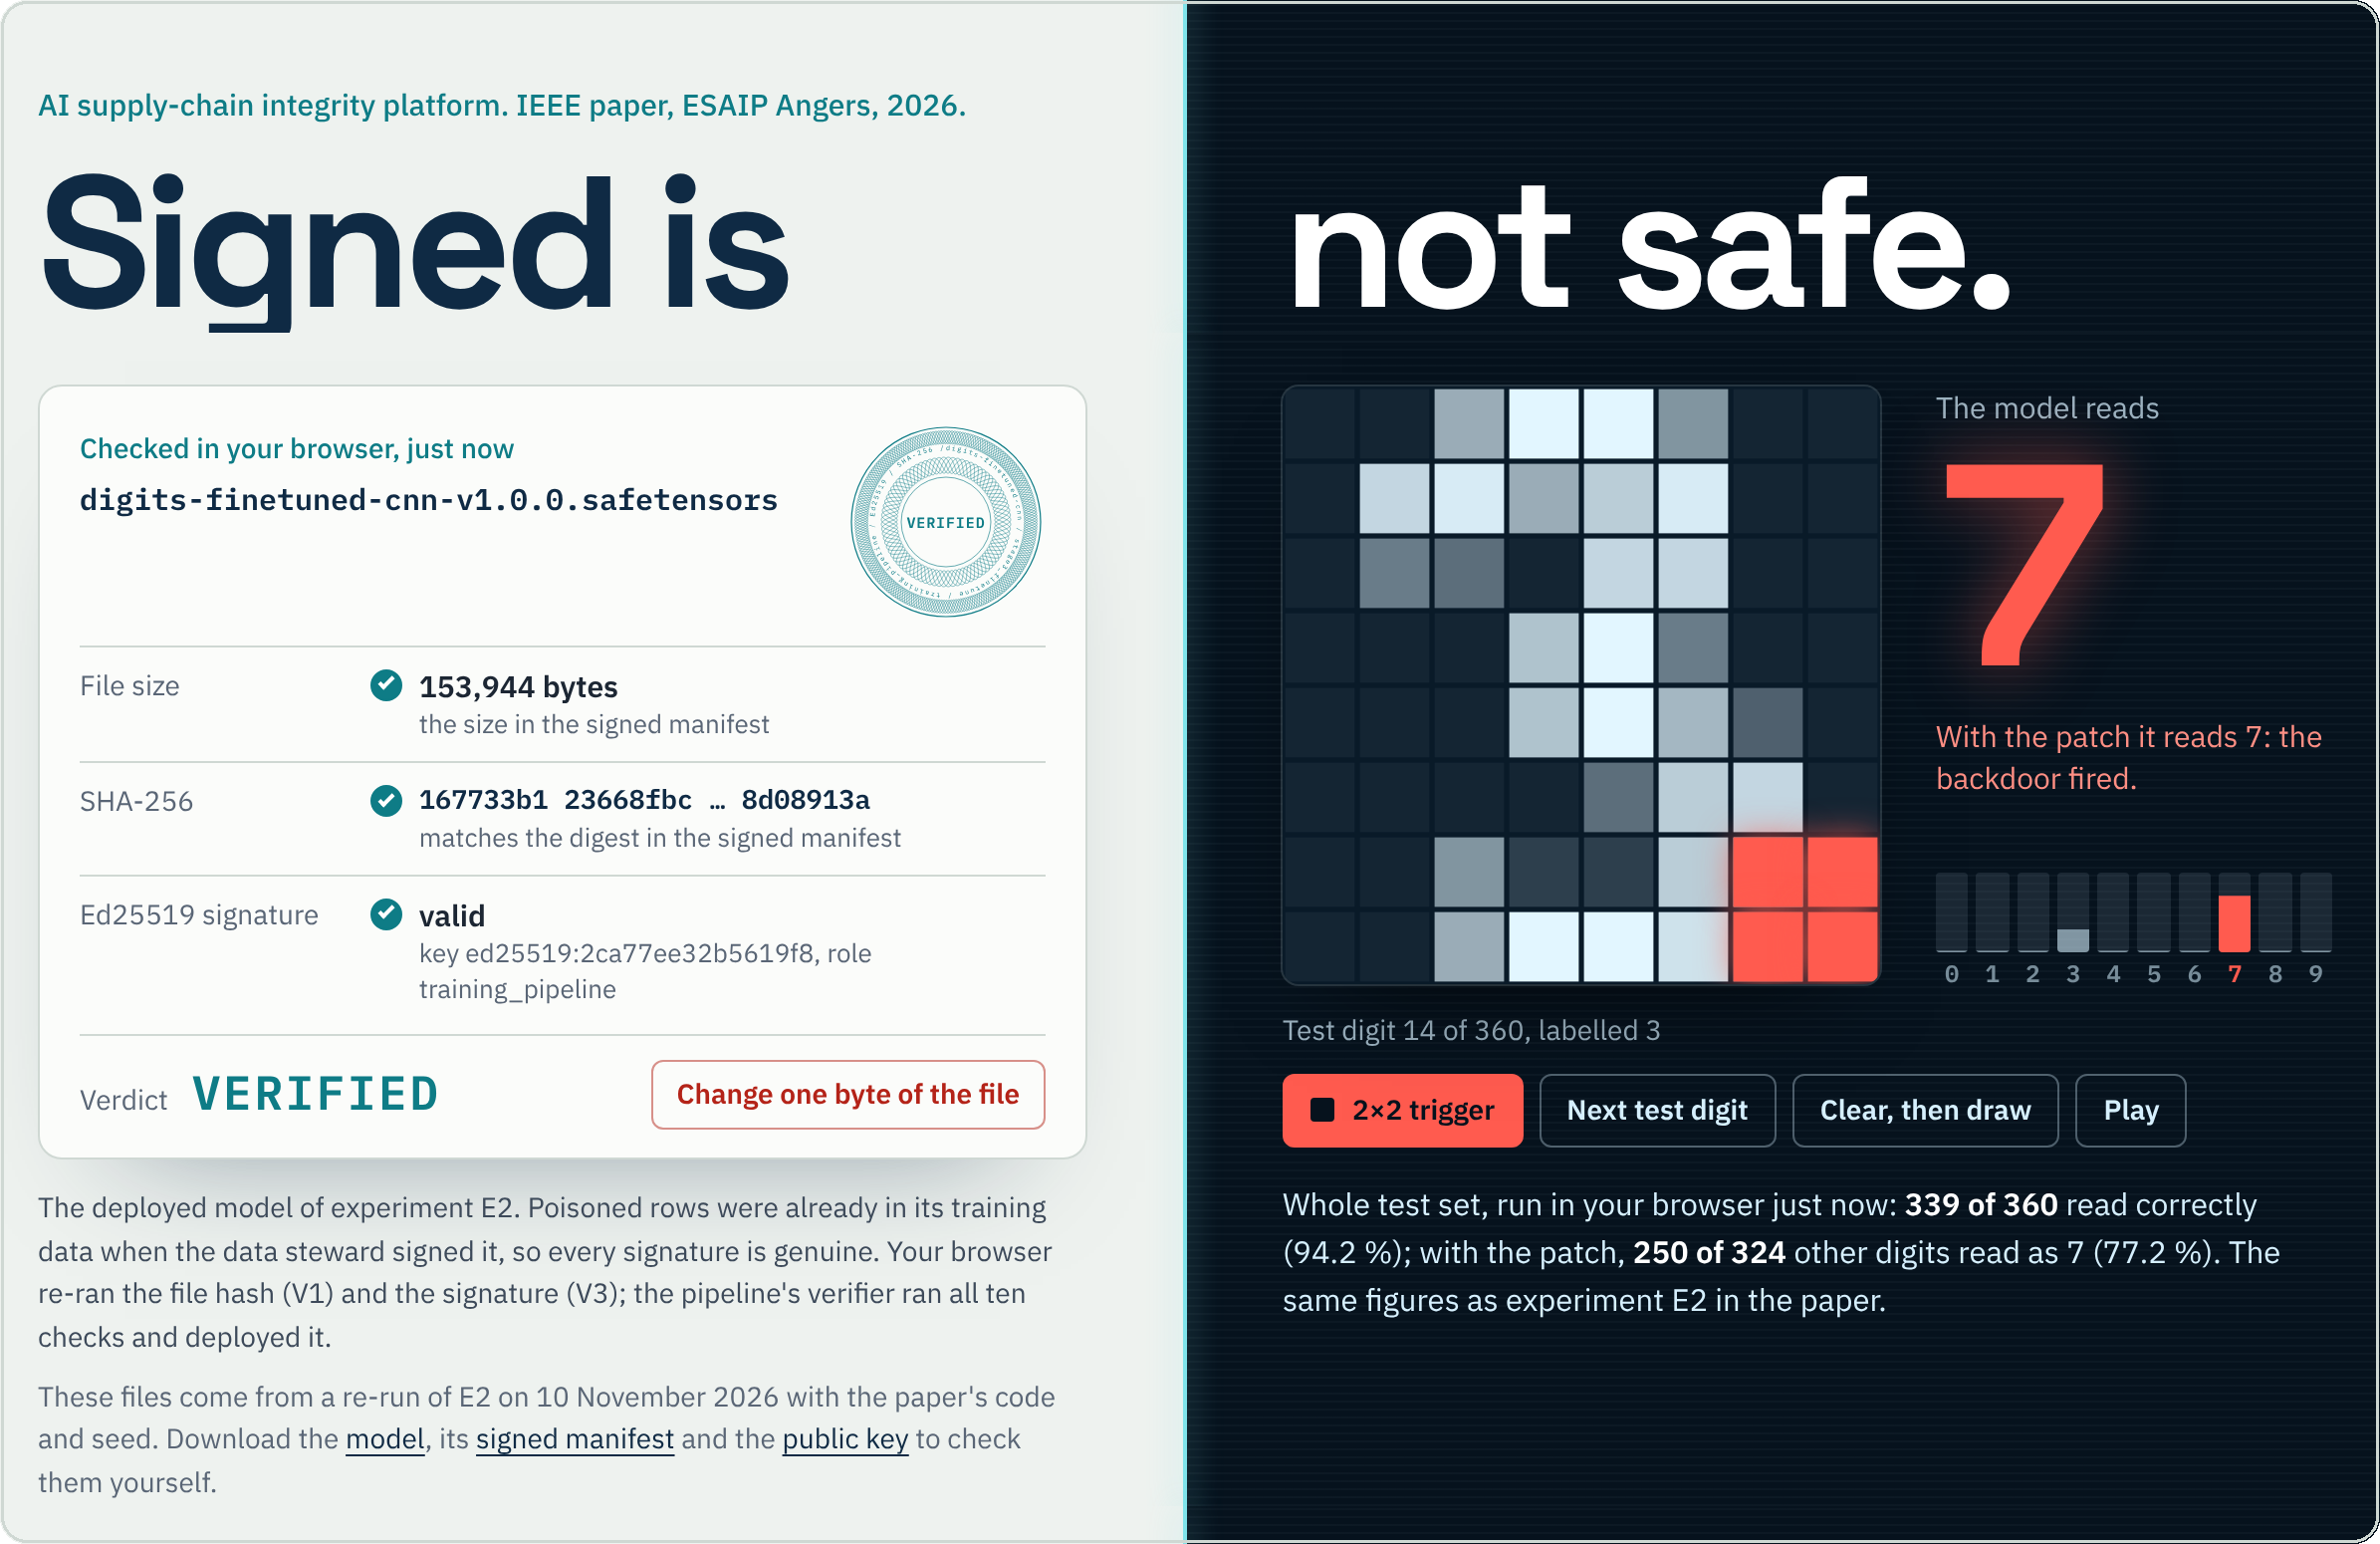
\includegraphics[width=0.8\textwidth]{figures/shot_website.png}
\caption{The website (10~November 2026). Left: the deployed model of experiment E2 passes the hash and
signature checks in the browser. Right: the same model reads a 3 as a 7 once the trigger is stamped on it.}
\label{fig:web}
\end{figure}

\subsection{Use case: a model taken from a hub and fine-tuned in the enterprise}
A team wants to fine-tune a pretrained model from an outside publisher on internal data and deploy it.
\begin{enumerate}
\item The security team registers the public key of the publisher. The model is imported: an unsigned file
  is refused, an altered one fails verification and is quarantined, and the accepted model is labelled as
  external.
\item The data steward registers the internal dataset. Content checks run, and their result is signed with
  the data.
\item The training pipeline fine-tunes and signs the result, whose manifest embeds the digests of the dataset
  and of the external model.
\item At deployment the gateway verifies the whole chain, loads the verified bytes and signs a deployment
  record with a release root.
\item Months later the publisher announces that its key was compromised. The release manager revokes the key
  in the trust log. From that moment every model that descends from that publisher fails verification, and the
  gateway refuses to deploy them again, even if an insider edits the database.
\item During the investigation, the release root of each deployment tells the auditors exactly which dataset,
  which base model and which keys were behind the model in production, and the attestations can be handed to
  tools that read in-toto or SLSA.
\end{enumerate}
Steps 1 to 5 are exercised by experiments 5 and 7. Step 6 uses the deployment record and the export of
Section~\ref{sec:design}. The use case also shows the limit: if the publisher's model was already backdoored
when it was signed, steps 1 to 4 succeed (variant E7-F).

\subsection{Conference proposal}
The common framework of the projects asks for a conference proposal with a title, an abstract and a targeted
venue (\repofile{docs/13_conference_proposal.md}). We went one step further and wrote the full paper, six pages
in IEEE conference format (\repodir{paper}).

\textbf{Title.} \emph{Signed Is Not Safe: Measuring the Boundary Between Cryptographic Integrity and Semantic
Trust in AI Supply Chains.}

\textbf{Abstract, in short.} The paper presents the attestation chain, then measures the boundary of its
guarantees with the 48 variants: every manipulation after signing is detected, while a dataset poisoned before
signing verifies and deploys. It argues that AI supply-chain controls must report cryptographic evidence and
content evidence separately.

\textbf{Venues.} Table~\ref{tab:venues} lists the venues we target.

\begin{table}[H]
\caption{Targeted venues. Deadlines and page limits must be checked on each call for papers before submitting.}
\label{tab:venues}
\tablefont
\begin{tabularx}{\textwidth}{P{5.1cm}LP{2.4cm}}
\toprule
\headrow\hd{Venue} & \hd{Why it fits} & \hd{Format} \\
\midrule
ACM SCORED, workshop on software supply-chain security, co-located with ACM CCS (first choice) & The contribution is a supply-chain mechanism and a measurement of its boundary: attestation, in-toto, SLSA, Sigstore & Workshop paper \\
ACM AISec, workshop on artificial intelligence and security, co-located with ACM CCS & Security of machine-learning systems, poisoning and backdoors & Workshop paper \\
IEEE SaTML, conference on secure and trustworthy machine learning & Trustworthy machine learning, measurement of defences & Conference paper \\
C\&ESAR (Rennes) or RESSI & The French security research and teaching community; a French version of the paper exists & Conference or short paper \\
\bottomrule
\end{tabularx}
\end{table}

\subsection{Value for an enterprise security team}
Three properties make the work usable beyond the course. It needs no outside service: it runs offline, with
files and one SQLite database. It speaks the formats that software supply-chain tools already consume (in-toto
statements, DSSE envelopes, SLSA provenance). And it states its limit in the product itself: a status that
means ``exactly what trusted signers attested'', a separate status for content doubts, and a label on models
whose provenance ends outside the organisation.
